\section{Reguladores}

Son elementos que mejoran el funcionamiento de la instalaci\'on, adaptando \'esta en cada momento a las necesidades reales.

\subsection{Regulador de presi\'on de evaporaci\'on}

Este regulador se monta en la tuber\'ia de aspiraci\'on, despu\'es del evaporador (\autoref{fig:instalacion-regulador-presion-evaporacion}), y se utiliza para mantener una presi\'on de evaporaci\'on constante y, por lo tanto, para mantener una temperatura constante en la superficie del evaporador. Protege contra una presi\'on de evaporaci\'on baja.

\begin{figure}[H]
    \centering
    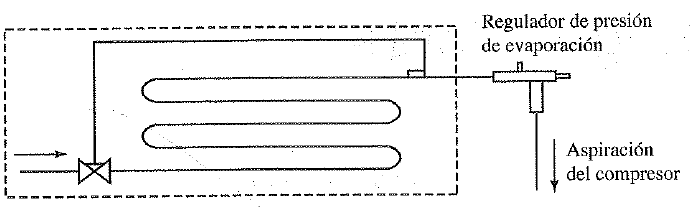
\includegraphics[width=.5\linewidth]{figuras/dispositivos-de-expansion/regulador-presion-evaporacion.png}
    \caption{Instalaci\'on del regulador de presi\'on de evaporaci\'on}
    \label{fig:instalacion-regulador-presion-evaporacion}
\end{figure}
\begin{wrapfigure}{r}{0.4\linewidth}
    \centering
    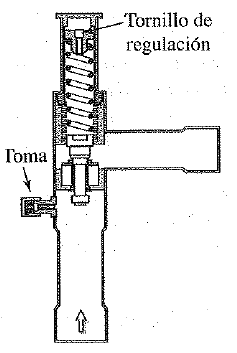
\includegraphics[width=.4\linewidth]{figuras/dispositivos-de-expansion/ajuste-regulador-presion.png}
    \caption{Ajuste del regulador de presi\'on}
    \label{fig:ajuste-regulador-presion}
\end{wrapfigure}
Para regularlo (\autoref{fig:ajuste-regulador-presion}) tiene una toma en la que se coloca un man\'ometro que nos indica la presi\'on a la entrada, es decir, la presi\'on en el evaporador. Mediante el tornillo de regulaci\'on variamos la presi\'on que ejerce el resorte y, con ello, la presi\'on de evaporaci\'on.

\textbf{Funcionamiento.}\ Cuando la presi\'on en el evaporador disminuye, el v\'astago se mueve restringuiendo el flujo y aumentando la presi\'on en el evaporador. En el caso contrario, el v\'astago deja pasar mayor flujo de refrigerante, disminuyendo la presi\'on en el evaporador.

Tambi\'en son utilizadas en aquellas instalaciones donde existen varios evaporadores a diferentes temperaturas, estas se montan a la salida de estos. Los circuitos a diferentes presiones se unen en el recipiente de l\'iquido, por lo tanto, para disgregar un circuito del otro se colocan valvulas antiretorno en los circuitos de menor presi\'on.

\subsubsection{Regulador de presi\'on de aspiraci\'on}

Este regulador se monta en la tuber\'ia de aspiraci\'on, antes del compresor. Protege al motor del compresor contra sobrecargas durante el arranque despu\'es de largos per\'iodos de parada o despu\'es de un desescarche.

Este regulador abre cuando disminuye la presi\'on de aspiraci\'on. Es decir, funciona seg\'un la presi\'on a la salida del regulador.

\subsubsection{Regulador de presi\'on de condensaci\'on}

En instalaciones que emplean condensadores por aire, cuando la temperatura del aire ambiente disminuye, por ejemplo en invierno, la presi\'on de condensaci\'on tambi\'en disminuye y el rendimiento de la instalaci\'on baja. Para evitar este inconveniente, se instalan estos reguladores (\autoref{fig:regulador-presion-condensacion}), ya que mantienen una presi\'on de condensaci\'on y de recipiente constantes. De otro modo se deber\'ia sobredimensionar la capacidad de la v\'alvula de expansi\'on.

\begin{figure}[H]
    \centering
    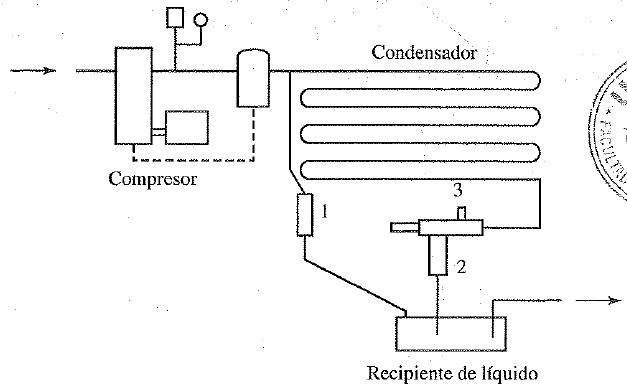
\includegraphics[width=.6\linewidth]{figuras/dispositivos-de-expansion/regulador-presion-condensacion.png}
    \caption{Instalaci\'on del regulador de presi\'on de condensaci\'on}
    \label{fig:regulador-presion-condensacion}
\end{figure}

En la instalaci\'on de la \autoref{fig:regulador-presion-condensacion}, al cerrar el regulador (2) con objeto de aumentar la presi\'on de condensaci\'on, la presi\'on en el recipiente disminuye por la alimentaci\'on de los evaporadores, con lo cual abrir\'ia la v\'alvula diferencial (1) y entrar\'ia en el recipiente vapor recalentado a alta presi\'on. La v\'alvula diferencial mantiene una diferencia de presi\'on entre la entrada del condensador y el recipiente de l\'iquido. El regulador abre al aumentar la presi\'on de entrada que es la presi\'on de condensaci\'on.

\subsubsection{Regulador de capacidad}

Los reguladores de capacidad se utilizan para mantener una carga uniforme en el compresor, independiente de la carga real del evaporador. Se instalan entre la aspiraci\'on y la descarga, uniendo \'estas (\autoref{fig:regulador-capacidad}).

Impide que la presi\'on de aspiraci\'on caiga por debajo de los valores establecidos. Cuando esto ocurre, la v\'alvula la abre y el vapor recalentador de descarga entra en la aspiraci\'on del compresor, elevando su presi\'on y, por lo tanto, aumenta su capacidad. 

\begin{figure}[H]
    \centering
    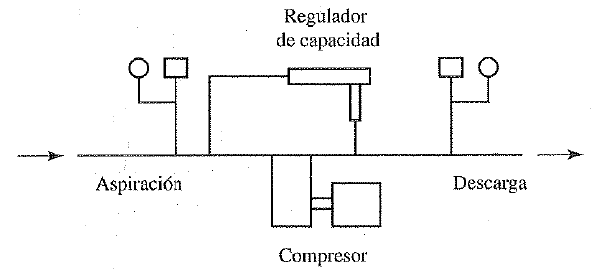
\includegraphics[width=.6\linewidth]{figuras/dispositivos-de-expansion/regulador-capacidad.png}
    \caption{Instalci\'on del regulador de capacidad}
    \label{fig:regulador-capacidad}
\end{figure}